%
% file: localoperator.tex
% author: Victor Brena
% description: Briefly describes properties of the local operator.
%

\chapter{Appendix A}
\label{app:app01}

\section{User Evaluation Survey}

\begin{figure}[H]
	\centering
	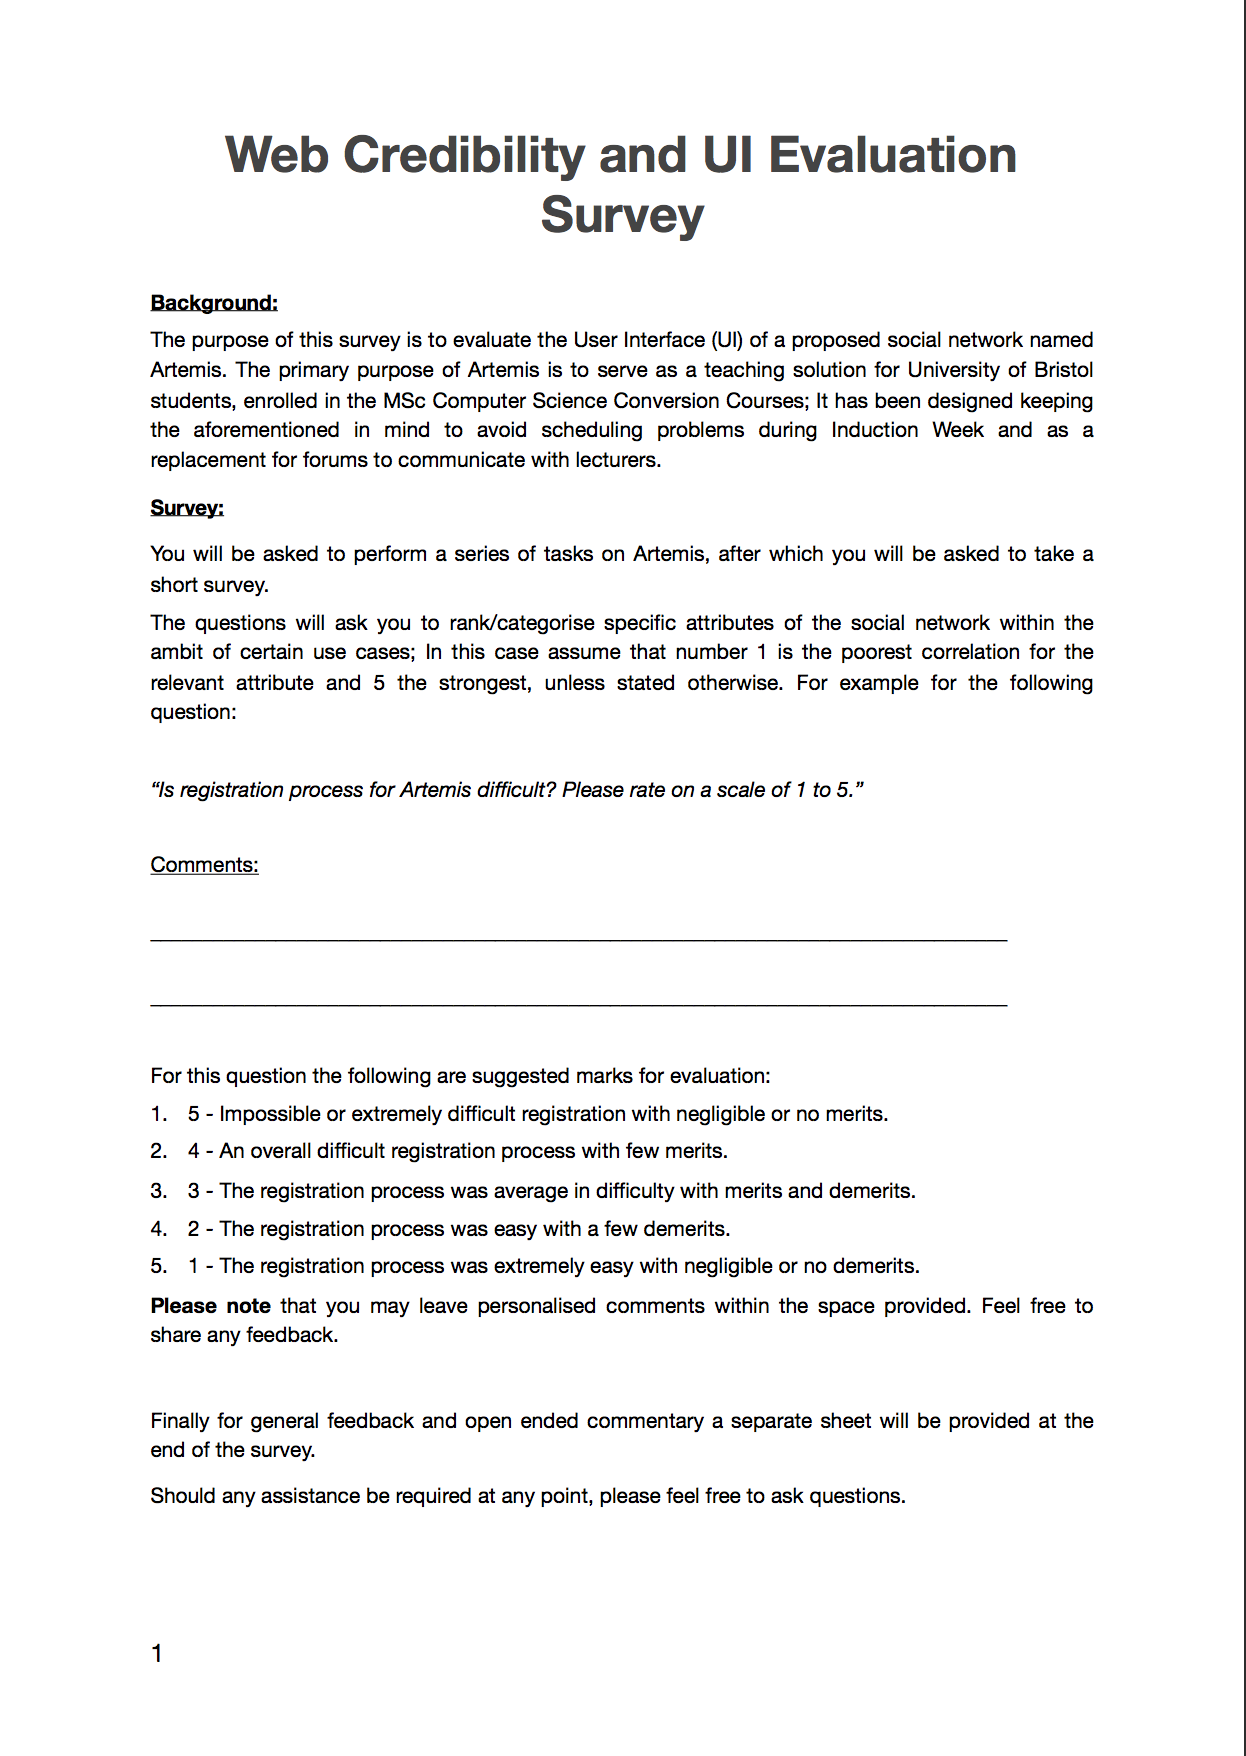
\includegraphics[scale=.60]{chapters/appendices/figures/1.png}
	\mycaption[User Evaluation Survey - 1/6]{User Evaluation Survey - 1/6}
	\label{fig:1/6}
\end{figure}
\newpage

\begin{figure}[H]
	\centering
	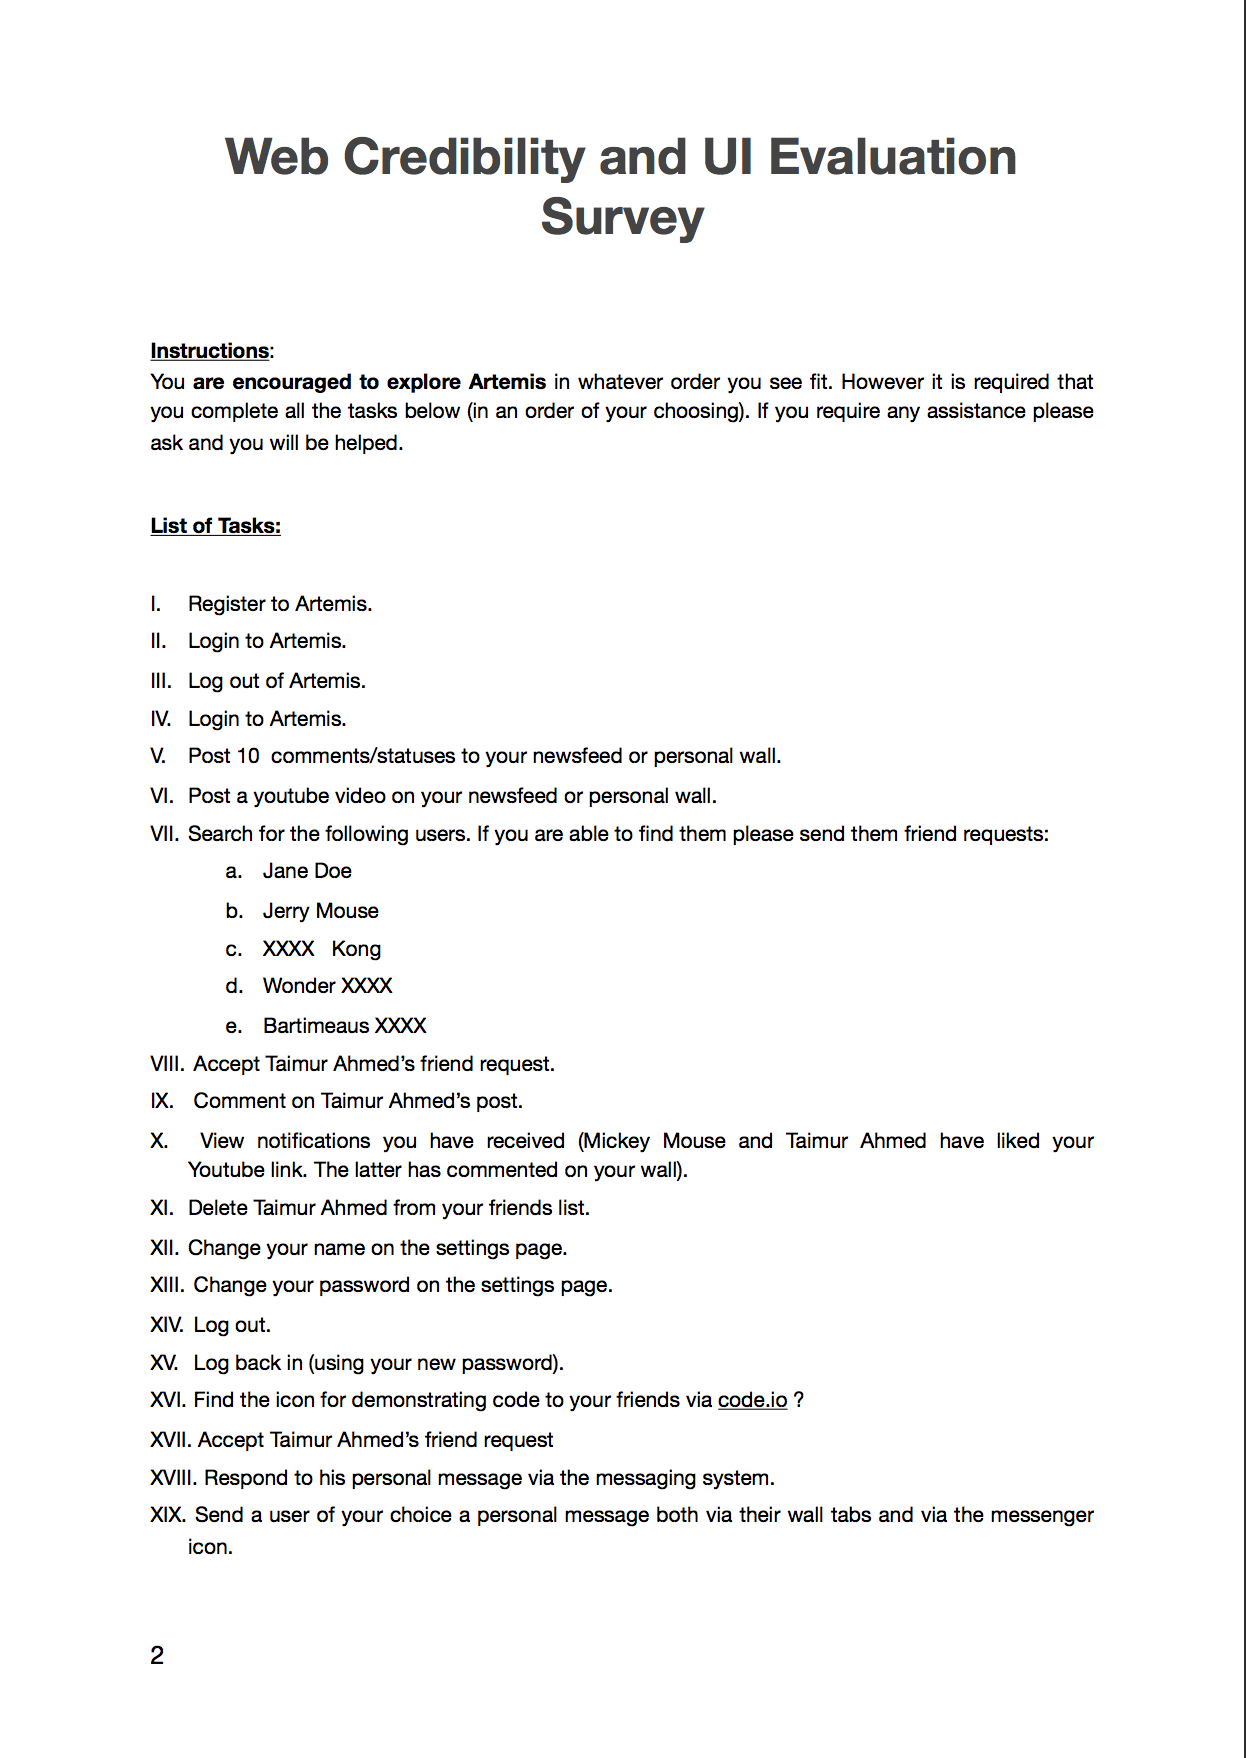
\includegraphics[scale=.7]{chapters/appendices/figures/2.png}
	\mycaption[User Evaluation Survey - 2/6]{User Evaluation Survey - 2/6}
	\label{fig:2/6}
\end{figure}
\newpage

\begin{figure}[H]
	\centering
	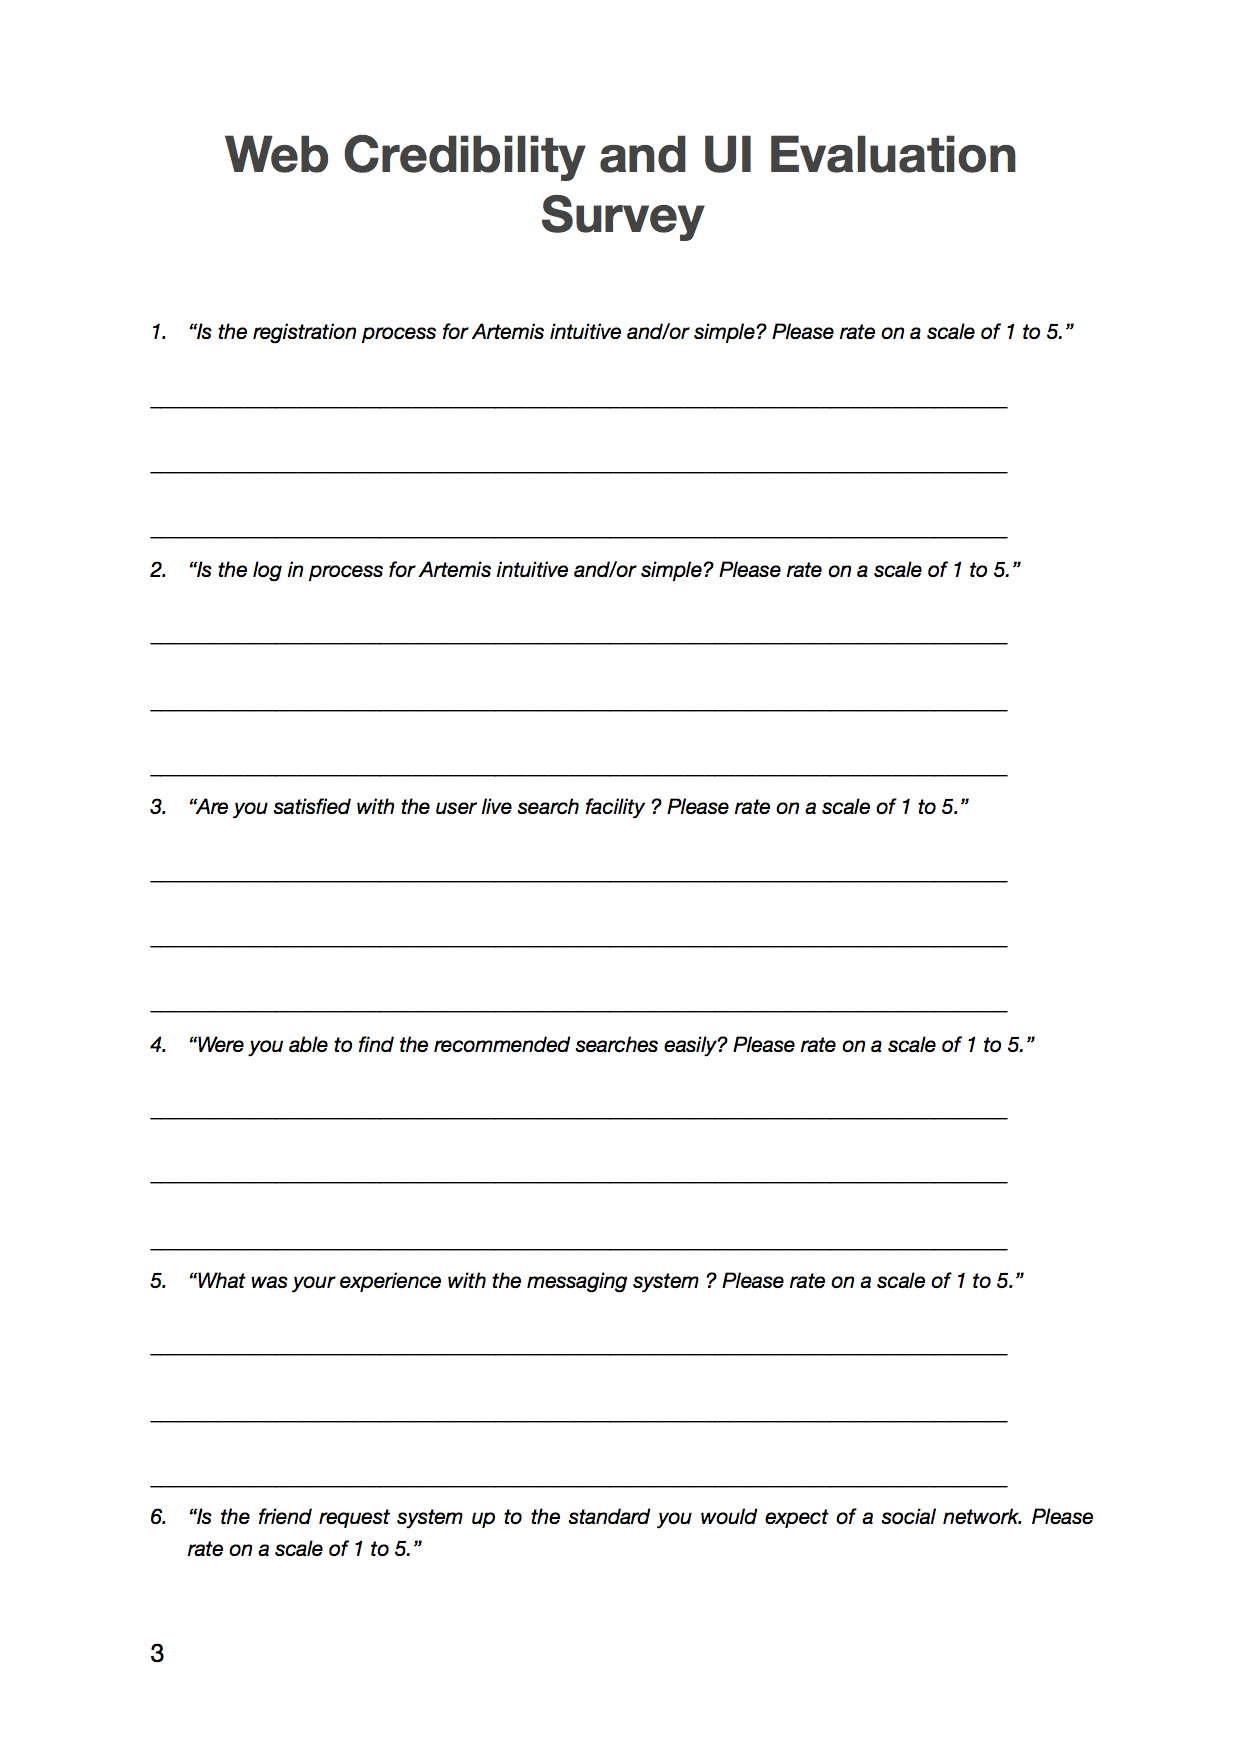
\includegraphics[scale=.7]{chapters/appendices/figures/3.png}
	\mycaption[User Evaluation Survey - 3/6]{User Evaluation Survey - 3/6}
	\label{fig:3/6}
\end{figure}
\newpage

\begin{figure}[H]
	\centering
	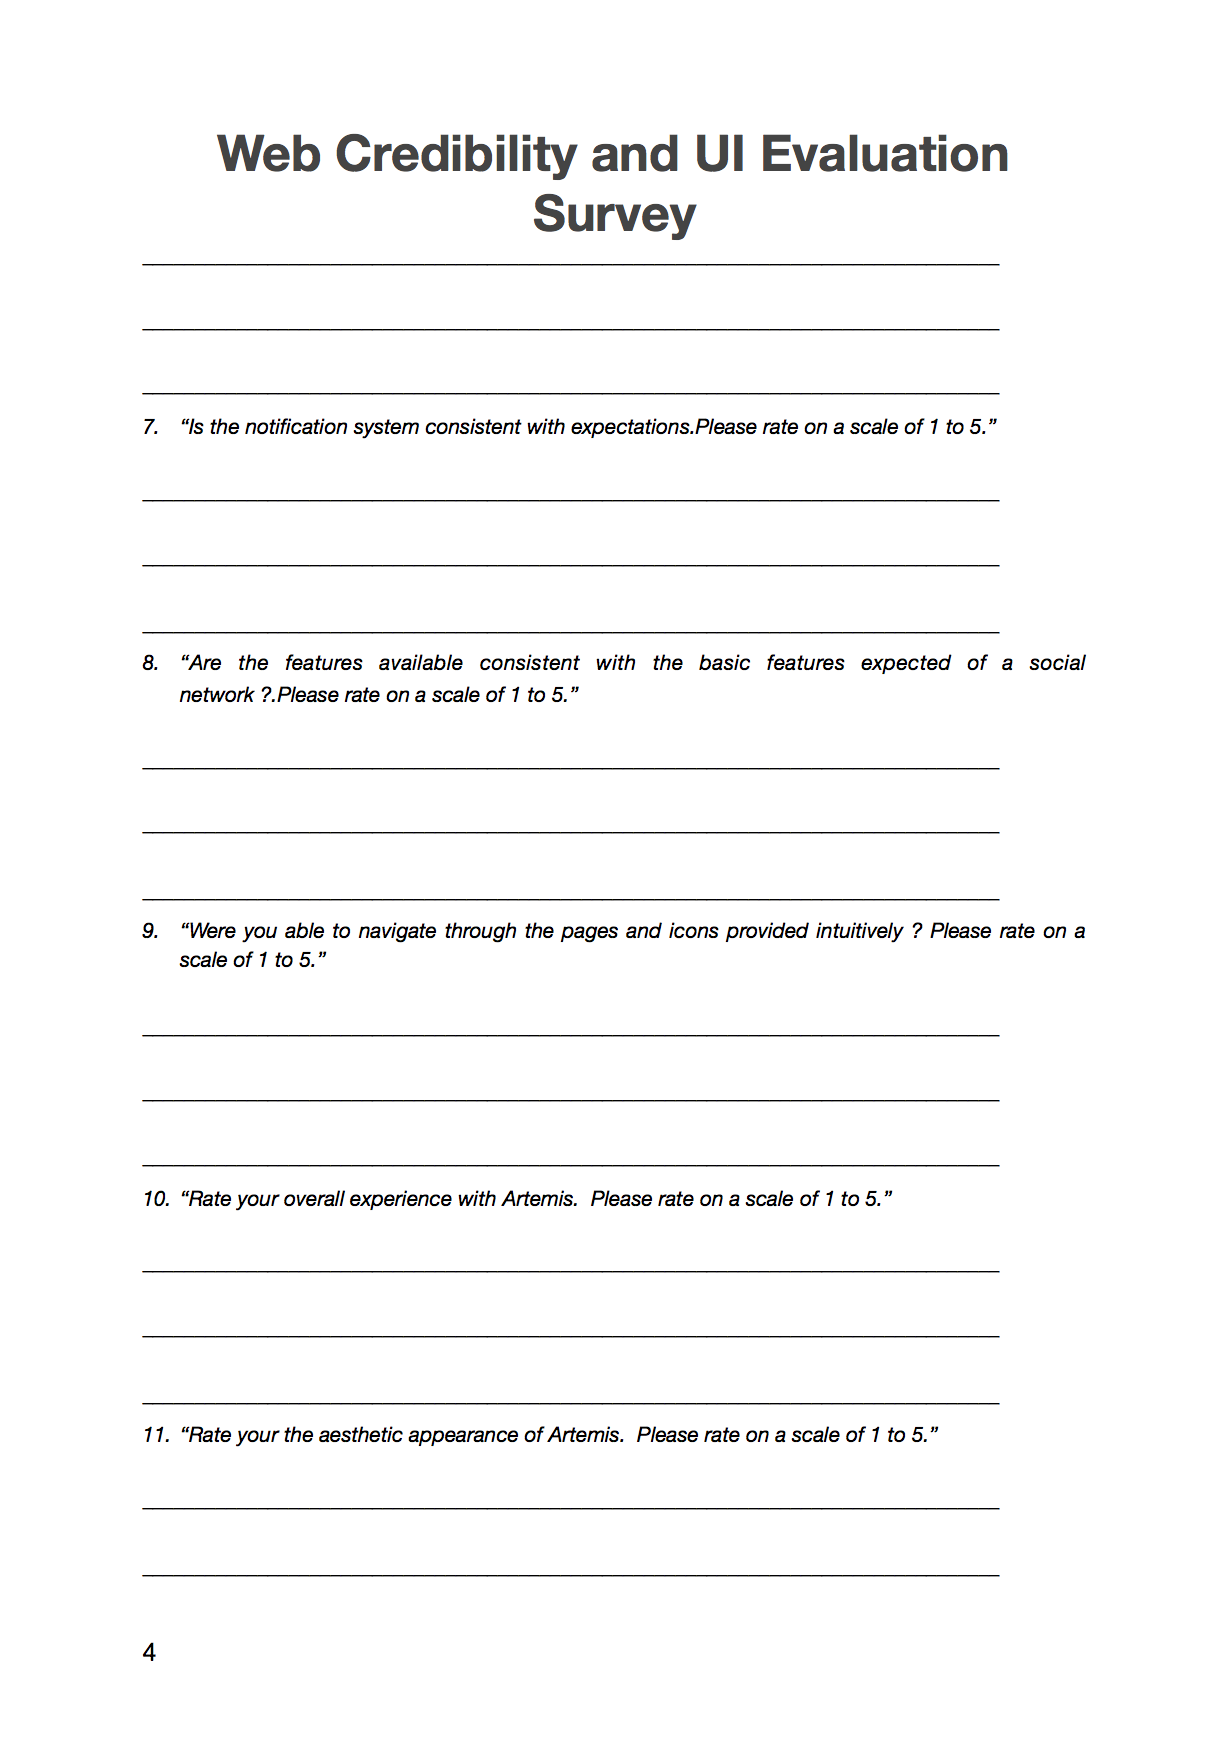
\includegraphics[scale=.7]{chapters/appendices/figures/4.png}
	\mycaption[User Evaluation Survey - 4/6]{User Evaluation Survey - 4/6}
	\label{fig:4/6}
\end{figure}
\newpage

\begin{figure}[H]
	\centering
	
\includegraphics[scale=.7]{chapters/appendices/figures/5.png}
	\mycaption[User Evaluation Survey - 5/6]{User Evaluation Survey - 5/6}
	\label{fig:5/6}
\end{figure}
\newpage

\begin{figure}[H]
	\centering
	
\includegraphics[scale=.7]{chapters/appendices/figures/6.png}
	\mycaption[User Evaluation Survey - 6/6]{User Evaluation Survey - 6/6}
	\label{fig:6/6}
\end{figure}
\newpage



\begin{landscape}
\section{The HTML Roles Data Model}
\begin{figure}[H]
	\centering
	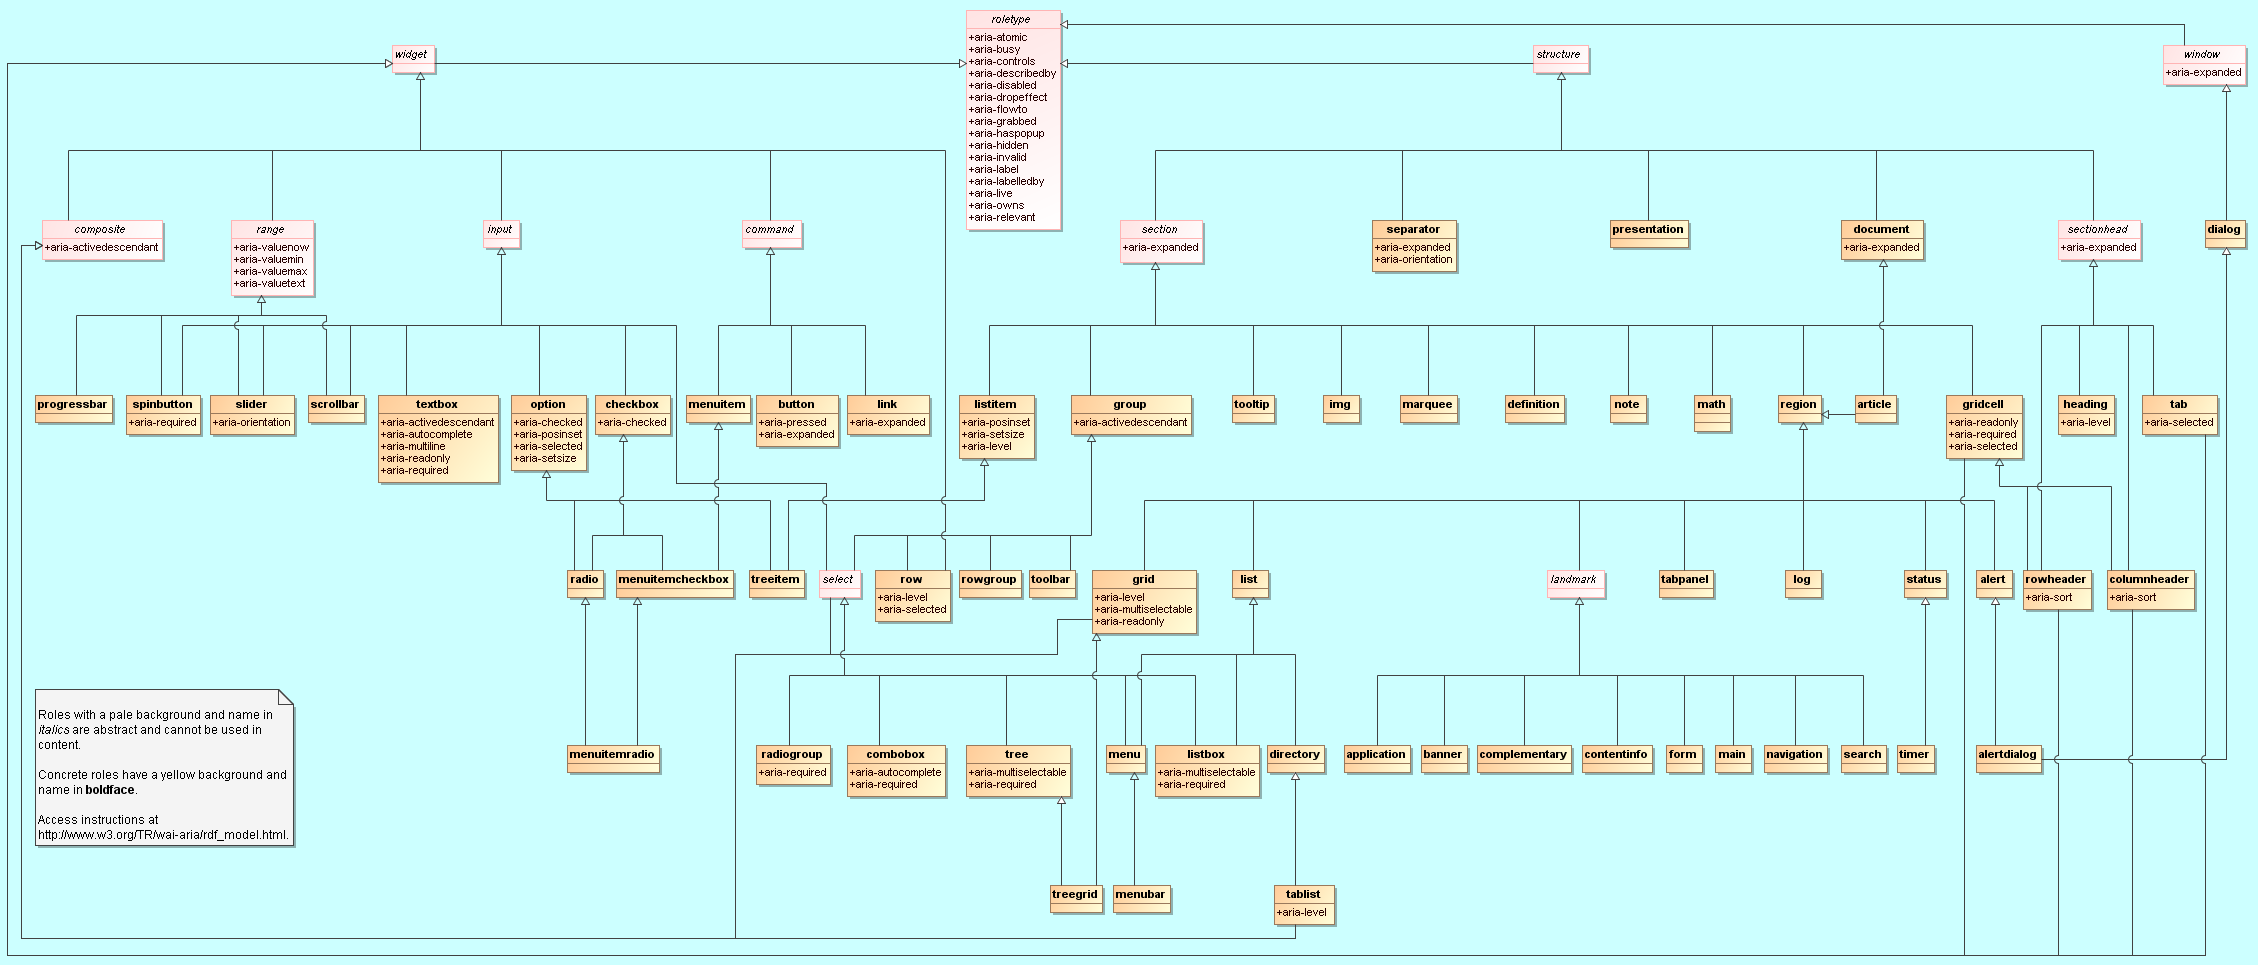
\includegraphics[scale=.29]{chapters/appendices/figures/rdf_model.png}
	\mycaption[Class diagram of the relationships described in the role data mode]{Class diagram of the relationships described in the role data mode}
	\label{fig:roleModelHTML}
\end{figure}
\end{landscape}